\chapter{Discussion}\label{ch:discussion}
\graphicspath{{../Figures/40-discussion/}}

{\doublespacing\normalsize\upshape
\noindent Publication note: Sections~\ref{sec:disc_effects}--\ref{sec:disc_bio} and the associated figures and tables appeared in \citet{bolen_2026} (Bolen, Elzein, Pang, and Hunt, \emph{Actuators}, 2026). Section~\ref{sec:disc_error} is also the subject of an unpublished manuscript in preparation by Bolen, Burgess, Morrow, Elzein, Pang, Scharzenberger, and Hunt \citep{bolen_isometric_2025}. This manuscript has not been submitted for publication. Author contributions for both works are stated in Chapter~\ref{ch:methods}.\par}


\section{Effects of Resting Length}\label{sec:disc_effects}
We have developed new $F_{620}$ equations for \qtylist{10;20}{\mm} diameter Festo BPAs that capture the change in maximum force produced by the actuators at  \qty{620}{\kPa} as a function of their resting length. When examining Equation~(\ref{eq:Fmax10}) and measured data in Figure~\ref{fig:Fmax_fit}b, it can be seen that as $l_0$ goes to infinity, $F_{620_{10}}$ goes to \qty{470}{\N}. When the Festo tool \citep{lang_robert_musclesim_2005} was queried at $l_0=\qty{1}{m}$ as an approximation of infinity, it predicts the $\phi$\qty{10}{\mm} BPA can produce $F=\qty{490}{\N}$ at $P_{620}$. This is within the 10\% variability that Festo states may occur in manufacturing tolerances. Similarly, the Festo data predict a $\phi$\qty{20}{\mm} BPA will produce $F=\qty{1570}{\N}$. Our results for Equation~(\ref{eq:Fmax20}) show that  $F_{620_{20}}$ goes to \qty{1460}{\N} as $l_0$ approaches infinity. Although the difference is much larger, it is also within the \mbox{10\% manufacturing tolerance. }

Our measured data differ significantly from the Festo model as $l_0$ goes to zero. For the measured data, as the length gets smaller, the force does as well, whereas the Festo tool predicts exponential force increase (see Figure~\ref{fig:Fmax_fit}). As a specific example, when specifying $l_0=\qty{112}{\mm}$ for the \qtylist{10}{\mm} diameter BPAs, the Festo predicted $F_{620}$ is \qtylist{498.6}{\N}. However, using Equation~(\ref{eq:Fmax10}), $F_{620}$ is calculated to be \qtylist{335.3}{\N}. Actual force in the $l_0=\qty{112}{\mm}$ was measured at \qtylist{350.9}{\N}. Therefore, the error in predicted $F_{620}$ for the $\phi$\qty{10}{\mm} BPA is $4.5\%$ for our model and $42.1\%$ using the Festo tool. Researchers using BPA resting lengths under \qty{300}{\mm} should take note of these results.

\citet{festo_2026} (p.~12) states that force will be reduced by approximately 10\% for a minimum nominal length. In \citet{festo_2018} (p.~14) they say the force can deviate by 10\% based on factors such as production variation, material variation, and deviation from nominal length ($l_0$). \citet{festo_2013} (p.~13) notes that testing was done with BPAs that are ten times the uninflated diameter, and that theoretical force can increase by up to 10\%. In each datasheet, the characteristic curves appear to be the same. As demonstrated above, the \qty{100}{\mm} $\phi$\qty{10}{\mm} BPA should have much less force than what is shown in the curve. This is our experience and the reason for the testing. It is unclear why the MuscleSIM tool \citep{lang_robert_musclesim_2005} then predicts higher force as resting length decreases. It could be a reversed sign coefficient in their internal curve-fit model. We have shown here that as the nominal length goes to zero, so does force. 

BPA models commonly predict higher forces than are measured experimentally because they do not account for end effects in regions of the pressure vessel where those effects dominate.	Nominally, the clamped ends fix the inner and outer diameter while allowing axial and radial displacement. In the isometric case, there is only radial displacement. The boundary conditions force steep gradients in stress and strain near the ends. Near the boundary conditions, axial, radial, and circumferential strains deviate from analytic solutions for a cylindrical model. For a constant pressure, the end effect region appears to have the same length. Therefore, in shorter BPAs, the end effects dominate. The axial length scale of the boundary section is comparable to $l_0$,  and the active force differs substantially from that of an assumed perfect cylinder.

Manufacturing variations seem to play an important role in the behavior of these actuators. It remains to be seen how $\epsilon_{620}$ can be known a priori. We still suspect that it is a function of $l_0$, but it might also be a function of other factors such as product batch number or UV light exposure \citep{festo_2026} (p.~15); \citep{festo_2018} (p.~6); \citep{festo_2013} (p.~13). We found there to be larger variations in the \qtylist{10}{\mm} BPAs than in the \qtylist{20}{\mm} BPAs. Modeling work on ideal McKibben actuators describes how the relationship between contraction and initial length is a function of the total number of twists and the angle of twist in the usable muscle area \citep{chou_measurement_1996}. It is unclear if there are variations in the angle and number of twists in the Festo BPAs due to manufacturing. Uncovering the relationship between $\epsilon_{620}$ and $l_0$ for the Festo DMSP artificial muscles, if it exists in a meaningful way, will require additional controlled tests. 

Similarly, it is not clear how the maximum force might change with manufacturing variations. This was reasonably corrected for by normalizing the equations to each individual's maximum contraction, but more nuanced details might emerge with more data collection. Not knowing these relationships a priori means there is still a need for robots and other systems to go through an iterative design stage if it is discovered that the system does not produce the torque or have the RoM that the design team expects. However, the data and models provided here should enable faster redesigns with fewer \mbox{additional measurements.}


\section{Nondimensionalized Force Prediction}

We have also introduced the concept of nondimensionalized isometric force that is a function of relative strain and relative pressure (Equation~(\ref{eq:Fstar})). This elegant equation has only three coefficients with low error (see Table~\ref{tab:Fstar}). In the work presented here, we introduce the relative pressure term, $P^*=P/P_{620}$. Our data show that by normalizing force, contraction, and pressure, we are able to create a simplified force equation as a function of contraction and pressure that scales well with initial actuator length, as expressed by Equation~(\ref{eq:force}) in Section~\ref{sec:force_model}.

For example, given $l_0=\qty{54}{\mm}$ and $P=\qty{300}{\kPa}$, the measured force was \mbox{$F_{actual} = \qty{103}{\N}$.} Force prediction using only the Festo tool predicts the force to be \mbox{$F_{predict} = \qty{270}{\N}$.} This is $161\%$ greater than the measured force. Using Equations~(\ref{eq:Fmax10}) and~(\ref{eq:Fstar}) with Equation~(\ref{eq:force}) gives $F_{predict} = F^*(0, 0.48) \cdot F_{620}(0.054) = 0.49 \cdot \qty{230}{\N} = \qty{112}{\N}$. This is an error of $8\%$, which is much more accurate than using the Festo tool only.

The presented work is capable of predicting force output for 10 mm and 20 mm muscles with different initial muscle lengths, internal pressure, and contraction amount with minimal initial data collection. However, it remains to be seen if these relationships are maintained over the full lifecycle of the muscles. There are not yet any peer reviewed studies investigating the long-term behavior of these artificial muscles, though the Festo datasheet provides some indication of what can be expected \citep{festo_2026} (p.19). They report that the 40 mm BPA can complete 1 million cycles at \qty{6000}{\N} (maximum rated load), or 10 million cycles at \qty{4000}{\N}. The service life of the other size BPAs is not reported; however, it is mentioned that thermal stressing may reduce the lifespan and they should be inspected every 500,000 cycles for signs of aging \citep{festo_2018} (pp.~10--11). Future research should look at the behavior of these muscles over time.

In our work, $P_{620}=\qty{620}{\kPa}$ is the maximum supply pressure for our system, and other users of this actuator may use a different supply pressure. However, this supply pressure is not required, and normalizing by this value was chosen as a method for improving the optimization techniques by reducing the sensitivity of the term associated with pressure. This equation will work for any pressure supplies below \qty{620}{\kPa}. We also anticipate the equation will also work for pressures up to \qty{800}{\kPa} (the maximum rated pressure for Festo $\phi$\qty{10}{\mm} BPAs); however, we do not have the data to confirm this.

\section{Comparison with Other Published BPA Models}

The proposed model was compared with the formulations by \citet{sarosi_new_2012}, \citet{sarosi_10mm}, and \citet{martens_modeling_2017}, to evaluate their predictive performance across actuator sizes and operating conditions (see Table~\ref{tab:model_compare} and Figure~\ref{fig:ModelCompare}).
For the $\phi$\qty{20}{\mm} BPA, parameters from \cite{sarosi_new_2012} were used, corresponding to actuators with resting lengths of \qty{200}{\mm} and \qty{400}{\mm}. These were compared against the experimental data at $l_0=\qty{300}{\mm}$ and $l_0=\qty{450}{\mm}$, respectively. For the $\phi$\qty{10}{\mm} BPA with resting lengths of \qty{257}{\mm} and \qty{233}{\mm}, parameters from \cite{sarosi_10mm} were applied. In each case, the maximum contraction parameter ($k_{max}$) was determined numerically by solving $F(\qty{6.2}{\bar}, k_{max}) = 0$, ensuring consistency with the experimental maximum pressure condition.




\begin{table}[H]
\caption{Goodness-of-fit comparison for the Bolen, Sárosi, and Martens and Boblan models at different resting lengths (in mm) for \qty{10}{\mm} and \qty{20}{\mm} BPAs. RMSE and maximum error are reported in newtons, and FVU denotes the fraction of variance unexplained.}
\label{tab:model_compare}
\tiny
\begin{adjustwidth}{-2cm}{0cm}
%\centering %% If there is a figure in wide page, please release command \centering
\begin{tabularx}{\textwidth}{@{}lllllllllll@{}}
\toprule
\textbf{Diameter} &
  \textbf{Length} &
  \textbf{} &
  \textbf{Bolen} &
  \textbf{} &
  \textbf{} &
  \textbf{Sarosi} &
  \textbf{} &
  \textbf{} &
  \multicolumn{2}{l}{\textbf{Martens and Boblan}} \\ 
\textbf{} &
  \textbf{} &
  \textbf{RMSE} &
  \textbf{FVU} &
  \textbf{Max. Error} &
  \textbf{RMSE} &
  \textbf{FVU} &
  \textbf{Max Error} &
  \textbf{RMSE} &
  \textbf{FVU} &
  \textbf{Max. Error} \\ \midrule
\textbf{10 mm} & 257 & 22.9 & 0.0353 & 46.0  & 143.8 & 1.3903 & 235.8 & 73.8  & 0.3668 & 122.9  \\
\textbf{}      & 233 & 16.8 & 0.0187 & 30.3  & 132.7 & 1.1655 & 222.6 & 62.6  & 0.2590 & 101.2  \\ \midrule
\textbf{20 mm} & 300 & 35.6 & 0.0144 & 114.0 & 132.1 & 0.1992 & 313.4 & 72.8  & 0.0605 & 137.8  \\
\textbf{}      & 450 & 67.6 & 0.0258 & 166.6 & 177.7 & 0.1785 & 294.8 & 862.1 & 4.2022 & 1321.1 \\ \bottomrule
\end{tabularx}
\end{adjustwidth}
\end{table}

While the \citet{sarosi_new_2012} and \citet{sarosi_10mm} models capture general trends in force–contraction behavior, discrepancies were observed when applying parameters derived from different actuator lengths. In particular, the model tends to over-predict force at higher pressures and low amounts of contraction, suggesting sensitivity to geometric scaling effects not explicitly accounted for in the formulation.

The \citet{martens_modeling_2017} model  is derived from a geometric and material-based framework and provides a more physically grounded representation of actuator behavior. However, its accuracy depends strongly on precise geometric parameters, including braid angle, wall thickness, and fiber length. Small deviations in these parameters can lead to significant differences in predicted force, particularly at higher pressures.

\begin{figure}[H]%[tbp]
%\begin{adjustwidth}{-\extralength}{0cm}
%\centering
%\begin{center}
    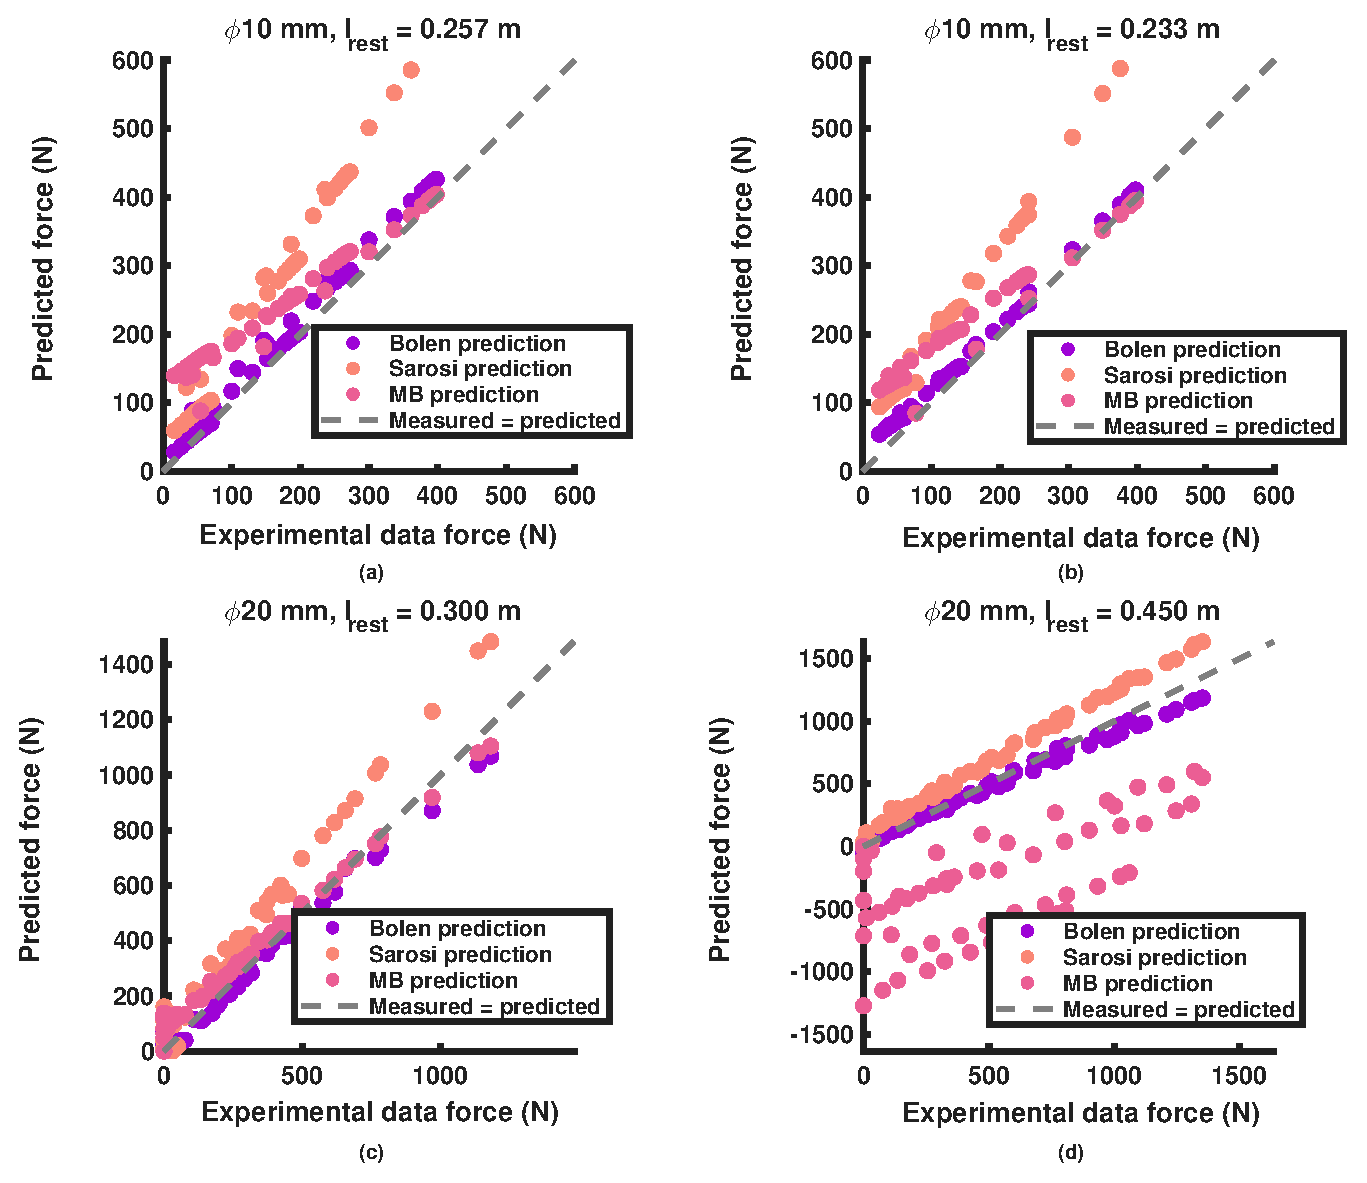
\includegraphics[width=.99\textwidth]{05_Comparison.eps}
%\end{center}
%\end{adjustwidth}
\caption{Comparison between measured and predicted BPA force at varying amounts of contraction and pressure. A $y=x$ perfect fit line is added for reference. The BPAs compared are: (\textbf{a}) $\phi$\qty{10}{\mm}, $l_0=\qty{0.257}{\mm}$, (\textbf{b}) $\phi$\qty{10}{\mm}, $l_0=\qty{0.233}{\mm}$, (\textbf{c}) $\phi$\qty{20}{\mm}, $l_0=\qty{0.300}{\mm}$, and (\textbf{d}) $\phi$\qty{20}{\mm}, $l_0=\qty{0.450}{\mm}$.}\label{fig:ModelCompare}
\end{figure}

The Martens and Boblan model was first evaluated at the same pressure–contraction points as in their experimental data \citep{martens_modeling_2017} (Tables A1 and  A2), indicating that it reproduces the general published force map shape but is sensitive to the assumed initial geometry. Examining their $\phi$\qty{20}{\mm} BPA, for example, using the explicitly stated $l_0=\qty{300}{\mm}$ and initial diameter $D_{0}=\qty{20}{\mm}$ significantly under-predicted the results compared to using the implied $l_0=\qty{296}{\mm}$ (\citep{martens_modeling_2017} (Table A1)) and $D_{0}+H_{0}=\qty{21.8}{\mm}$, where $H_{0}=\qty{1.8}{\mm}$ is the material thickness. The diameter adjustment can be inferred \mbox{from \citep{chou_measurement_1996}.} This adjusted diameter was also included for the $\phi$\qty{10}{\mm} BPA to give a better fit. As can be seen in Figure~\ref{fig:ModelCompare} and Table~\ref{tab:model_compare}, the highest accuracy is observed when $\phi$\qty{20}{\mm} and $l_0=\qty{300}{\mm}$, which is at or very near their experimental measurements. For the $\phi$\qty{10}{\mm} BPAs the accuracy decreases even though their experimentally measured $l_0=\qty{250}{\mm}$ is close to our $l_0=\qty{257}{\mm}$ and $l_0=\qty{233}{\mm}$. The largest error occurs at $\phi$\qty{20}{\mm} and $l_0=\qty{450}{\mm}$ and the model starts to predict negative force. We have calculated that the $F_{PE}\cdot\frac{dD}{DL}$ term becomes very large compared to the others \citep{martens_modeling_2017} (p.~5). This suggests that the model is sensitive to geometric parameter selection and interpretation, particularly with respect to initial length and diameter definitions.

In comparison, the present normalized model demonstrates improved consistency across actuator lengths by incorporating experimentally derived scaling through $F_{620}$ and $\epsilon_{620}$. This normalization reduces sensitivity to geometric variation and enables a unified representation of actuator behavior, while maintaining predictive accuracy over the tested range of pressures and contractions.


\section{Implications for Real-Time Control and Simulation}

Although pneumatic muscle actuators exhibit hysteresis, thermodynamic effects, and other dynamic behavior, accurate and high-performance controller designs can still be achieved using a static force map approach when the underlying static force model is accurate. Martens and Boblan explicitly note that BPA dynamics are often dominated by the air dynamics inside the actuator and the mass flow behavior of the valve, such that precise modeling of the static force characteristic remains crucial for torque control \mbox{accuracy \citep{martens_modeling_2017}.} This view is consistent with more recent BPA control work, including a sensor-less torque control interface for BPA-driven joints \citep{martens_framework_2018}, stable force/position/stiffness control of antagonistic pneumatic-muscle joints \citep{ugurlu2019stable, hunt_development_2017}, and sensor-less angle stiffness control of antagonistic BPA systems \citep{shinSensorlessAngleStiffness2022}. 

In this context, the present model is well suited for real-time use because it reduces the static isometric force prediction to a low-order normalized surface, $F^*(\epsilon^*,P^*)$, scaled by the resting-length-dependent term $F_{620}(l_0)$. This structure is computationally inexpensive to evaluate online and is also suitable for lookup-table implementation. While the present work does not model the full actuator--valve dynamics, it provides the static force relationship needed as a feedforward or inner-model component in real-time torque control, simulation, and preliminary design workflows. It is anticipated that improved real-time control for high-speed and high-precision systems will benefit more from improved modeling of airflow dynamics than from modeling actuator hysteresis, damping, and other dynamic behavior. Characterizing the actuators under dynamic operating conditions --- isokinetic (constant-velocity), isobaric, and isotonic (constant-load) contractions --- is a natural next step beyond the isometric characterization reported here, for which the pressure--force dynamics model of \citet{elzein_pressure_2025} provides the modeling foundation.



\section{Biomimetic Artificial Muscle Analogy}\label{sec:disc_bio}

BPA artificial muscles are often said to be analogous to biological muscles because they have force--length curves and can produce force only in tension. This analogy is worth closer inspection. For example, the passive force–length curve has been described as an exponential function arising from connective tissue elements, while the active force–length relationship is typically modeled as a bell-shaped curve reflecting actin–myosin overlap \citep{winters1990}. These formulations emphasize that muscle force generation is governed by nonlinear geometric and material interactions rather than simple linear elasticity.
McKibben-type pneumatic artificial muscles (of which Festo is an example) exhibit analogous nonlinear behavior, though arising from fundamentally different physical mechanisms. As shown by Chou and Hannaford, the force–length relationship of McKibben actuators is derived from geometric constraints imposed by the braided shell, leading to a nonlinear dependence of force on actuator length through the braid angle \cite{chou_measurement_1996}. In their formulation, actuator force is proportional to pressure and a nonlinear geometric term $(3\cos^2\theta - 1)$, which governs both the maximum contraction limit and the curvature of the force–length relationship. The work presented here demonstrates that this nonlinear curve can be well approximated by an exponential as well.

However, the behavior of these artificial muscles differs distinctly from that of biological muscles.
For example, the optimal fiber length of a biological muscle, $l_{OFL}$, is not equivalent to $l_0$ in an artificial muscle. Artificial muscles produce their maximum active force at their resting length, which is also their maximum length. In contrast, the maximum active force that a biological muscle can produce is somewhere in the middle of the total contractile length of the muscle. 

Furthermore, biological muscles can adapt the optimal operating length through structural remodeling (e.g., sarcomere addition or tendon compliance) while BPAs have a fixed geometric configuration. This allows biological systems to self-optimize for the particular tasks the animal is subjected to. In order to re-optimize a robot for new tasks, new actuators would have to be swapped into the system. This distinction highlights a key limitation of BPAs in biomimetic applications, while also reinforcing the importance of accurate nonlinear modeling for control and design.




\section{Sources of Error in Isometric Torque Generation}\label{sec:disc_error}

Our improved BPA characterization predicts torque more accurately than the original BPA model (see Fig.~\ref{fig:FlxPin_group}\textbf{A} and \ref{fig:FlxPin_group}\textbf{B}). This only accounts for part of the error. There are certainly many factors that affect the torque results. Compliance in the testing system, positioning tolerances, flexibility of brackets, imperfect path modeling, and variation in individual BPAs are other factors.

Simplifying and testing the model revealed deficiencies in our previous analysis. The isometric system is not rigid. There is compliance in the winch cable, artificial tendons, and brackets that bend and stretch. We introduced a constant length offset term $\chi_{0}$, axial stiffness $\chi_{1}$, and bending stiffness $\chi_{2}$. The bracket frame of reference was placed at the onset of the cantilevered section and rotated about $Z$.  The optimization identified parameter values for a $\phi$\qty{10}{\mm} BPA with $l_{0}=\qty{48.5}{\cm}$ in the simple pinned knee configuration. These results were validated with a second $\phi$\qty{10}{\mm} BPA with $l_{0}=\qty{45.7}{\cm}$.

The modeling of extensor BPA paths that wrap around the knee joint is an approximation with inherent error (Fig. \ref{fig:Ext_passthru}). When the moment arm is short, small changes to it can have a large effect on the resultant torque \citep{young_analyzing_2019}. It was assumed that wrapping the BPA around the joint would be easier to account for than adding a patella, deterministically designing its location as a function of knee angle, and accounting for friction. At greater knee flexion angles, shorter $l_{0}$ BPAs were observed to stretch and compress (see Fig.~\ref{fig:testJigs}\textbf{C}). The same loading sometimes caused the BPA to slip off the anterior head of the bolt that holds the femur to the knee. This produced a $\pm \; 20\,\text{mm}$ displacement in the $Z$ direction, changing both the force vector and the torque. The system designer, too, must be mindful. Fig. \ref{fig:ExtPin_group} shows a deviation between measured and originally predicted results that widens as expected torque increases. This indicates system compliance. However, the hybrid-calculated torque matches or exceeds the predicted torque, except at greater flexion angles for the $l_{0}=\qty{41.5}{\cm}$ BPA, indicating a loss of functional $l_m$; this is why the $\chi_{3}$ term was created in \eqref{eq:deltaL}. Fig. \ref{fig:ExtPin_group} shows the improved fit from running the optimization that includes this term.

The biomimetic knee joint with an extensor BPA was used to validate the extensor optimization results. The corrected prediction more closely matches the measured torque values, although it remains higher than the measurements.


The nonlinear biomimetic robotic system presented here replaces rigid-body simplifications commonly used in other robotic and biomechanical systems. Instead, progressing from simple to complex systems elucidated compliance mechanisms that can lead to more accurate first-iteration designs. Technologies have been developed to predict system bending and axial compliance, a constant length offset, and a loss of usable length that occurs as artificial muscle bends around a joint. 

In equation $m\ddot \varepsilon^* + c (\dot \varepsilon^* ) \dot \varepsilon^* + k ( \varepsilon^* ) \varepsilon^* = F$ given $k(\varepsilon^{*}, P^{*})
= \left.\frac{\partial F}{\partial \varepsilon^{*}}\right|_{P^{*}}
= -c_{0}c_{1}e^{-c_{1}\varepsilon^{*}}
  - 2c_{2}\varepsilon^{*}P^{*}e^{-c_{2}(\varepsilon^{*})^{2}}$
then if we set mass m and external force F to zero we get
$c (\dot \varepsilon^* ) = (k ( \varepsilon^* ) \varepsilon^*)/\dot \varepsilon^*$


\section{Synthesis: From Actuator Characterization to Neuromechanical Control}\label{sec:synthesis}

Taken together, the actuator and joint level results of this dissertation form a coherent design chain for biomimetic legged robots. At the actuator level, the maximum isometric force of Festo BPAs was shown to depend strongly on resting length, correcting a systematic over-prediction by the manufacturer's tool at short resting lengths, and a nondimensional force surface was derived that predicts isometric force from relative strain and relative pressure with only three diameter-dependent coefficients. At the joint level, the improved actuator model was combined with a compliance-corrected musculotendon kinematics model to predict isometric knee torque across the full range of motion for pinned and biomimetic knee joints, and the biomimetic knee driven by optimized BPAs was shown to meet or exceed human isometric torque over most of the range of motion.

This chain was developed deliberately so that each stage can feed the next. The force model supplies the actuator terms for the torque model; the torque model supplies the biomechanical model for designing joint controllers; and the validated biomimetic knee demonstrates that the actuator architecture can reproduce human joint-level force capabilities. The neural layer is no longer only a proposal: the OpenSim-to-MuJoCo conversion, BPA coupling interface, SNS-Toolbox spinal architecture, sensory channels, and staged validation workflow described in Sections~\ref{sec:preliminary_sim_methods}--\ref{sec:preliminary_sim_results} provide a working framework for neuromechanical experiments. The AARL's prior AnimatLab walker (Section~\ref{sec:prior_walker}) explains why that framework emphasizes systematic verification: its hand-tuned two-layer CPG produced gait-like suspended stepping, but its afferent feedback did not generalize to weight-bearing motion. Chapter~\ref{ch:futurework} therefore presents closed-loop quantification, ground-robustness comparisons, and hardware transfer as independent research programs enabled by the completed framework.

The cross-platform verification campaign (Sections~\ref{sec:crossengine_methods}--\ref{sec:bpa_walker}) adds a design constraint that runs through this chain: a synthetic nervous system is a mathematical object, and it must survive translation between the tools in which it is built, verified, and deployed. Reproducing the contact-driven rhythm core with exact period agreement and trace correlations above 0.9999 between independent NumPy and Simulink implementations --- with the archived AnimatLab models reproducing their published rhythms headless in the same protocol --- establishes that the SNS formalism, not any particular simulator, carries the dynamics. The persistent-sodium half-center with a fixed inactivation time constant, the graded synapse, and contact-driven rhythm are therefore portable primitives: they can be tuned in whichever engine is fastest and trusted in whichever engine is most physical. The campaign's negative results are equally structural. The feedforward CPG of the prior walker and the contact-driven core of the W2L architecture sit at deliberate, opposite points of the sensory-dependence spectrum --- the former oscillates without feedback but could not bear weight, while the latter will not oscillate at all without phasic heel feedback, a load dependence that echoes the decerebrate-cat locomotion of Section~\ref{sec:bg_neural}. The missing piece for unsupported walking is balance --- a network layer, not an engine feature --- and the BPA-actuated walker's peak forces at 60\% of the pressure ceiling indicate that, once that layer exists, the actuation margin is already there.

% [ZCODE 2026-10-02 Spiking-mirror campaign BEGIN — additive goal-4 dissertation edit. Source of truth: Code/MuJoCo_SNS/spinal/reports_spiking_20261002 (gated campaign). Results: Section~\ref{sec:spiking_results}. Nothing above this fence was changed.]
\section{What Spiking Changes and Does Not}\label{sec:disc_spiking}

The spiking-mirror campaign (Sections~\ref{sec:spiking_methods} and~\ref{sec:spiking_results}) allows the dissertation's neural-coding assumption to be examined directly, and its outcome divides cleanly into what the coding regime changes and what it leaves alone.

What spiking does not change is the plant-side behavior, provided the hybrid doctrine and the calibration hold. Because the motor-neuron layer stays non-spiking and the spikes onto it are calibrated by mean conductance, the interface that the actuator and torque models of this dissertation attach to --- a continuous activation command per muscle --- is unchanged by construction. The Simulink twins make the point quantitatively: with only the sensory interneuron layer converted, the knee-reflex transient is identical, the settle band moves by \ang{0.9}, and the beverage-holding reflex modulation moves by \ang{0.02}. To the plant, a calibrated \qty{40}{\hertz} train and the graded voltage it replaces are the same command; the activation dynamics of the muscle model filter the spike train the same way the biological membrane would. The actuator-level and joint-level conclusions of Chapters~\ref{ch:methods}--\ref{ch:results} therefore do not depend on the neural coding chosen above the motor-neuron layer.

What spiking changes first is timing. The mirror's self-sustained rhythm runs \qty{55.6}{\percent} slower than the analog build at the same constant drive, and its air-stepping cadence is roughly ten times faster than the non-spiking twin's in that preparation --- deviations in opposite directions in the two tests, which is itself informative, since a single scaling error would move both the same way. The campaign traced the constant-drive period to two identifiable knobs, the threshold-increment magnitude and the adaptation time constant, and demonstrated alternation/period trade-offs along them; the untuned starting point, not a structural failure, is the honest reading. Any period-matched spiking controller is therefore a short tuning campaign away, and the mirror's mapped parameters are the correct starting point for it.

What spiking changes second is robustness, in the mirror's favor. The analog network's constant-drive rhythm sits close to a bifurcation --- an exact port of it to a different integration stack can settle to the tonic fixed point --- so marginal winners risk not surviving a solver change. The spiking half-centers passed the perturbation basin gate in full, with the rhythm persisting under \qty{1}{\percent} jitter on every scalar parameter including the spiking-specific ones, at $0.89\times$ of the baseline swing. For the hardware-transfer program of Chapter~\ref{ch:futurework}, where the network will be re-implemented on embedded hardware with finite-precision arithmetic, a rhythm whose basin is wide is the safer substrate, and the sub-stepping cost of resolving spikes (\qty{0.5}{\milli\second} network steps inside the unchanged \qty{2}{\milli\second} plant step) is modest.

What spiking does not tolerate is a naive parameter port at the synapse level. The AnimatLab conversions show that converting graded synaptic amplitudes to per-spike increments of the same magnitude breaks the reciprocal half-center loop outright --- the loop is either starved of inhibitory charge or saturated --- while converting only the thresholds changes nothing, and the 2023 spiking walker of the same lineage walks because it was tuned as a rate code from birth. Synaptic strength in a spiking network is a rate-code quantity that must be derived from the presynaptic firing rate and the conductance decay, exactly as the MuJoCo mirror's calibration script derives it, not copied from the graded value. This is the one place where the campaign's negative results should temper expectations: spiking conversion is an exercise in re-derivation, and the calibration-first, gate-everything procedure of Section~\ref{sec:spiking_methods} is the transferable method.

Finally, the one place where the untuned spiking mirror outperforms its tuned non-spiking twin --- producing a bilateral ground gait where the winner's left leg is frozen --- is a single run with no statistics, and it is claimed only as a lead. But it points at the mechanism the hybrid doctrine was after: the mirror's afferents are event-coded, its adaptation is spike-history-based, and its inhibitory charge arrives in discrete quanta, so the phase relationships that the analog build locks in around a frozen leg are not the only stable operating regime of the same topology. Establishing whether that regime survives tuning, and whether event-coded contact afferents are what unlock it, is precisely the closed-loop CPG comparison program defined in Chapter~\ref{ch:futurework}, and the mirror is now the instrument for running it.
% [ZCODE 2026-10-02 Spiking-mirror campaign END]

% [ZCODE 2026-10-03 Pulley-route discussion + FLAG-BEN torque-test placeholder BEGIN — additive edit anchored after sec:disc_spiking. Sources: Mesh_Optimization/Results/{Bifemsh_20mm_Result.mat, Bifemsh_20mm_Result_pulley_20260926_1652.mat, BiPulley_batch_summary.csv, BiPulley_opensim_bifemsh_r_20260926_1702.mat} via the 2026-10-03 session digest; the pulley results have no counterpart in 30-results.tex yet, so every number below is digest-cited. Nothing above this fence was changed.]
\section{What Mono- and Bi-Pulley Routing Buys}\label{sec:disc_pulley}

The route redesign of Section~\ref{sec:ongoing} placed both \qty{20}{\mm} actuators on direct attachment routes. The Mono/Bi-pulley algorithms extend that search space by allowing the artificial tendon to be reeved over pulleys before insertion, and the flexor pulley run of 2026-09-26 quantifies what the added routing freedom is worth on the knee-flexor route of record. The pulley variant converged to a collision-feasible layout with zero bound violations (pattern-search exit flag 1) at an objective of 0.08465 under its own objective function, which differs from the direct route's objective of 74.47, so the two values are not commensurable. The best configuration on file reeves the two actuators over a single tackle-line part at a gain fixed at 1:1, so the pulley acts as a redirect rather than a force multiplier; even so, the redirect alone deepened the peak predicted flexion torque from \qty{81.23}{\newton\cdot\meter} to \qty{85.74}{\newton\cdot\meter}, a gain of \qty{4.51}{\newton\cdot\meter} (\qty{5.6}{\percent}), while holding the off-axis torque to at most \qty{0.803}{\newton\cdot\meter}, under \qty{1}{\percent} of the peak on-axis value; the predicted peaks of the direct and pulley routes exceed the human flexor torque scale of \qty{23.16}{\newton\cdot\meter} by factors of 3.51 and 3.70. The Bi-pulley batch establishes where that freedom runs out on anatomical routes. Across the five OpenSim muscle sites attempted (soleus, tibialis anterior, rectus femoris, medial gastrocnemius, and biceps femoris short head), every run closed with a nonpositive torque margin (objectives of 0.929 for tibialis anterior, 0.997 for soleus, and 3.42 for rectus femoris with a residual worst-constraint value of 0.242), and the medial-gastrocnemius and biceps-femoris-short-head runs terminated at the infeasibility sentinel (objective 101, worst-constraint value 10, exit flag $-2$). For the four runs that report a finite route-to-route clearance, the binding constraint was geometry rather than torque: minimum pair clearances spanned \qty{4.26}{\mm} to \qty{19.14}{\mm} against the \qty{25}{\mm} separation required between adjacent routes (two \qty{10}{\mm} actuator radii plus a \qty{5}{\mm} bundle margin); the medial-gastrocnemius run records no finite clearance, so its failure rests on the infeasibility sentinel alone. What the two algorithms buy is therefore reach and screening: the mono-pulley converts routing freedom into \qty{4.51}{\newton\cdot\meter} of additional predicted flexion torque without mechanical advantage and with off-axis torque below \qty{1}{\percent} of the peak, and the bi-pulley sweep screens candidate anatomical sites, showing that its reeved routes do not yet fit these corridors and redirecting the design effort toward clearance-relaxed attachment sites. These pulley solutions are optimizer-stage results; they have not yet been propagated into the OpenSim or MuJoCo model trees used for the simulation work of Sections~\ref{sec:preliminary_sim_methods}--\ref{sec:preliminary_sim_results}, and the hardware torque tests of the updated compliant system are pending, so the block below is reserved for their results.

% FLAG-BEN 2026-10-03: PENDING torque-test results for the updated compliant system (the physical redesigns returned by Opt_run.m / Opt_run_Ext.m under the adopted correction terms of Section~\ref{sec:ongoing}). The pending claim is NOT stated as fact anywhere in this chapter. TODO(Ben): replace the bracketed placeholder below with the measured torque-versus-angle numbers (flexor and extensor, worst-margin angles, pressures) once the runs land, then delete this comment pair.
\noindent\textit{[FLAG-BEN, PENDING TORQUE-TEST RESULTS: Once the pending torque-test runs land, this paragraph will state that the updated compliant system lets \texttt{Opt\_run} and \texttt{Opt\_run\_Ext} meet or exceed human torque magnitude, and it will report the measured torque-versus-angle results for the redesigned flexor and extensor routes. TODO(Ben): insert the measured numbers.]}
% [ZCODE 2026-10-03 Pulley-route discussion + FLAG-BEN torque-test placeholder END]
